\chapter*{Gabarito}

\section*{Capítulo 1 - Afinal, o que é um robô?}

    \subsection*{1)}
    Pergunte ao professor
        \begin{multicols}{3}
            \begin{figure}[H]
            \caption{Praticar esportes}
     
            \centering 
            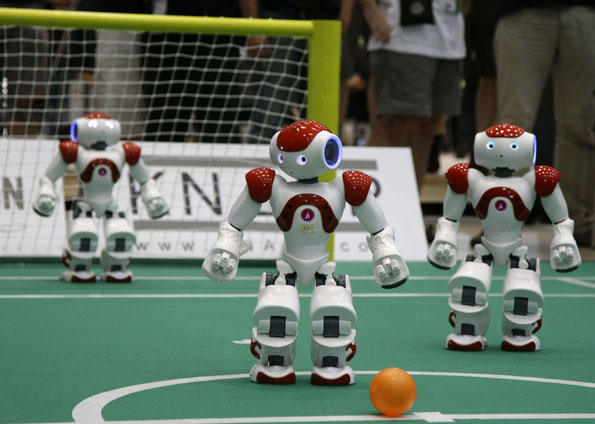
\includegraphics[width=5cm]{Figuras/NAU.jpg}
            \label{figura:NAU.jpeg}
            \end{figure}
        
            \begin{figure}[H]
            \caption{Robô que anda em terra e na água, pode ser utilizado para localizar coisas}
     
            \centering 
            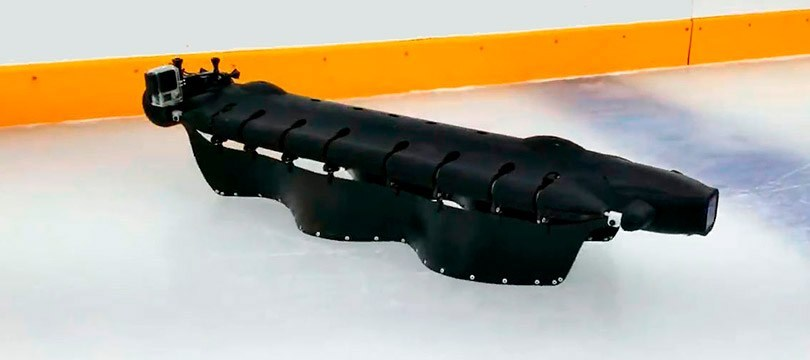
\includegraphics[width=5cm]{Figuras/anfibio.jpg}
            \label{figura:garcom.jpeg}
            \end{figure}

            \begin{figure}[H]
            \caption{Sophie, estudos sobre inteligência artificial}
     
            \centering 
            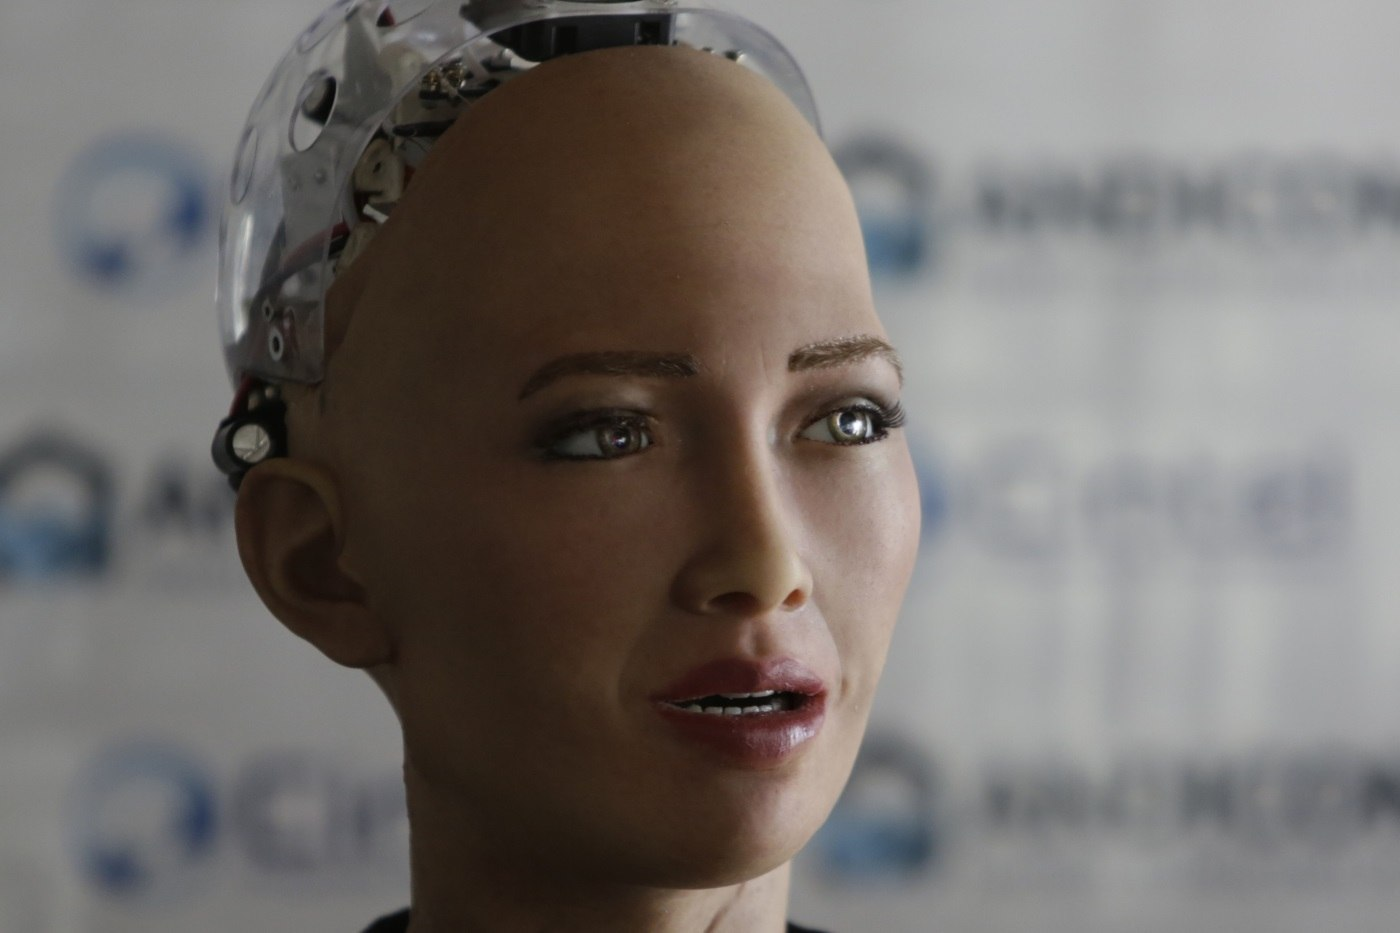
\includegraphics[width=6cm]{Figuras/sophie.jpeg}
            \label{figura:sophie.jpeg}
            \end{figure}
        \end{multicols}
        
     \subsection*{2)}
        Não, termômetros não são capazes de tomar decisões, de agir sobre o meio, ele é somente uma ferramenta para calcular e visualizar a temperatura ambiente.
        
    \subsection*{3)} Pergunte ao professor
        
    \subsection*{4)}
        A geladeira sabe quando a porta está aberta e quando está fechada, e nisso decide se acende ou apaga a luz de dentro dela, porém isso não passa apenas de algum circuito lógico. Uma boneca que fala ou se mexe sozinha é bem "robótica" por dentro, mas é incapaz de perceber os seus arredores e realizar ações não repetitivas (tenha certeza que o fabricante disse que a boneca deveria se mexer, caso não venha explicitado, pode ser caso de assombração!).
        
    \subsection*{\textbf{Desafio}}
        Pergunte ao professor
        
        
\section*{Capítulo 2 - Algoritmos e tela LCD}

    \subsection*{1)}
    

    
    \subsection*{2)}
    

    
    \subsection*{3)}
    
    \subsection*{4)}

    
    \subsection*{Desafio) Perguntar ao professor.}

\section*{Capítulo 3 - Movimentação}

    \subsection*{1)}
    Letra c.
    
    \subsection*{2) (Existe mais de uma solução para este exercício)}

    \begin{minted}{cpp}
    #include <Sparki.h>
    void setup ()
    {
    }
    void loop ()
    {
        sparki.moveForward(5);
        sparki.moveRight();
    }
    \end{minted}
    
    \textsl{Como a distância a ser percorrida pelo robô é equivalente ao lado do quadrado, o valor dentro dos parênteses da função ``sparki.moveForward()'' é 5.}
    
    \subsection*{3) (Existe mais de uma solução para este exercício)} 
    
    \begin{minted}{cpp}
    #include <Sparki.h>
    void setup ()
    {
    }
    void loop ()
    {
        sparki.moveForward(500);
        sparki.moveRight();
    }
    \end{minted}
    
    \textsl{Como o lado do quadrado passou a ser 5 metros, é necessário transformar esse valor para centímetros antes de escrever dentro dos parênteses da função.}
    
    \subsection*{4)}
    Letra d.
    
    \subsection*{5)}
    
    \begin{minted}{cpp}
    #include <Sparki.h>
    void setup ()
    {
    }
    void loop ()
    {
        sparki.moveForward(500); //anda 5 metros para frente
        sparki.moveRight(90); //olha para a direita
        sparki.moveLeft(180); //olha para a esquerda
        sparki.moveRight(90); //volta a olhar para frente
    }
    \end{minted}

    \subsection*{6)}
    \textsl{Este código abre totalmente as garras e depois as fecha durante 1 segundo. Poderia simular as garras pegando um objeto.}
    
    \subsection*{Desafio) Perguntar ao professor.}
    
\section*{Capítulo 4 - Ultrassom}

    \subsection*{1)}
    
        Conhecendo a velocidade do som, nós sabemos quantos centímetros o som percorre em 1 segundo, se conhecermos também quanto tempo levou para a onda ir e voltar, fazendo uma \textbf{regra de três} podemos descobrir quantos centímetros a onda andou, então é só dividir esse valor pela metade que temos a distância até o objeto mais próximo.
    
    \subsection*{2)}
    
    \begin{minted}{cpp}
    #include <Sparki.h>
    int distancia;
    void setup()
    {
    }
    void loop()
    {
        distancia = sparki.ping();
        delay(500);
        sparki.clearLCD();
        sparki.print(distancia);
        sparki.updateLCD();
    }
    \end{minted}
    
    \subsection*{3)}
    
    \begin{minted}{cpp}
    #include <Sparki.h>
    void setup()
    {
        sparki.servo(SERVO_CENTER);
        delay(3000);
    }
    void loop()
    {
        sparki.servo(SERVO_LEFT);
        delay(800);
        sparki.servo(SERVO_RIGHT);
        delay(800);
    }
    \end{minted}
    
    \subsection*{4)}
    
        \begin{minted}{cpp}
    #include <Sparki.h>
    int distancia;
    void setup()
    {
        sparki.servo(SERVO_CENTER);
        delay(500);
    }
    void loop()
    {
        distancia = sparki.ping();
        delay(500);
        distancia = distancia - 7;
        sparki.moveForward(distancia);
        delay(3000);
    }
    \end{minted}
    
    \subsection*{Desafio) Perguntar ao professor.}

\section*{Capítulo 5 - Variáveis}

    \subsection*{1)}
    
    \subsection*{2)}
    
    \subsection*{3)}
    
    \subsection*{4)}
    
    \subsection*{5)}
    
    \subsection*{Desafio) Perguntar ao professor.}

\section{Capítulo 6 - If e Else}

    \subsection*{1)} Letra b.
    
    \subsection*{2) (Existe mais de uma solução para este exercício)}
    
    \begin{minted}{cpp}
    #include <Sparki.h>
    void setup()
    {
        int x = 2042385;
    }
    void loop()
    {
        sparki.clearLCD();
        if(!(x % 2)) {
            sparki.print("O numero e par.");
        } else {
            sparki.print("O numero e impar.");
        }
        sparki.updateLCD();
        delay(1000);
    }
    \end{minted}
    
    \subsection*{3)}
    
    \subsection*{4)}
    
    \subsection*{5)}
    
    \subsection*{Desafio) Perguntar ao professor.}

\section*{Capítulo 7 - Infravermelho}

    \subsection*{1)}
    
    \subsection*{2)}
    
    \subsection*{3)}
    
    \subsection*{4)}
    
    \subsection*{5)}
    
    \subsection*{Desafio) Perguntar ao professor.}
    